\documentclass[a4paper,14pt,oneside,final]{extarticle}
\usepackage[top=2cm, bottom=2cm, left=3cm, right=1cm]{geometry}
\usepackage{scrextend}

\usepackage[T2A,T1]{fontenc}
\usepackage[ukrainian,russian,english]{babel}
\usepackage{tempora}
\usepackage{fontspec}
\setmainfont{tempora}

% Зачем: Отключает использование изменяемых межсловных пробелов.
% Почему: Так не принято делать в текстах на русском языке.
\frenchspacing

\usepackage{indentfirst}
\setlength{\parindent}{1.25cm}
\renewcommand{\baselinestretch}{1.5}

% Header
\usepackage{fancyhdr}
\pagestyle{fancy}
\fancyhead{}
\fancyfoot{}
\fancyhead[R]{\small \selectfont \thepage}
\renewcommand{\headrulewidth}{0pt}

% Captions
\usepackage{chngcntr}
\counterwithin{figure}{section}
\counterwithin{table}{section}
\usepackage[tableposition=top]{caption}
\usepackage{subcaption}
\DeclareCaptionLabelFormat{gostfigure}{Рисунок #2}
\DeclareCaptionLabelFormat{gosttable}{Таблиця #2}
\DeclareCaptionLabelSeparator{gost}{~---~}
\captionsetup{labelsep=gost}
\captionsetup[figure]{labelformat=gostfigure}
\captionsetup[table]{labelformat=gosttable}
\renewcommand{\thesubfigure}{\asbuk{subfigure}}

% Sections
\usepackage[explicit]{titlesec}
\newcommand{\sectionbreak}{\clearpage}

\titleformat{\section}
  {\centering}{\thesection \quad}{0pt}{\MakeUppercase{#1}}
\titleformat{\subsection}[block]
  {\bfseries}{\thesubsection \quad #1}{0cm}{}

\titlespacing{\section} {0cm}{0cm}{21pt}
\titlespacing{\subsection} {\parindent}{21pt}{0cm}
\titlespacing{\subsubsection} {\parindent}{0cm}{0cm}

% Lists
\usepackage{enumitem}
\renewcommand\labelitemi{--}
\setlist[itemize]{noitemsep, topsep=0pt, wide}
\setlist[enumerate]{noitemsep, topsep=0pt, wide, label=\arabic*}
\setlist[description]{labelsep=0pt, noitemsep, topsep=0pt, leftmargin=2\parindent, labelindent=\parindent, labelwidth=\parindent, font=\normalfont}

% Toc
\usepackage{tocloft}
\tocloftpagestyle{fancy}
\renewcommand{\cfttoctitlefont}{}
\setlength{\cftbeforesecskip}{0pt}
\renewcommand{\cftsecfont}{}
\renewcommand{\cftsecpagefont}{}
\renewcommand{\cftsecleader}{\cftdotfill{\cftdotsep}}

\usepackage{float}
\usepackage{pgfplots}
\usepackage{graphicx}
\usepackage{multirow}
\usepackage{amssymb,amsfonts,amsmath,amsthm}
\usepackage{csquotes}

\usepackage{listings}
\lstset{basicstyle=\footnotesize\ttfamily,breaklines=true}
\lstset{language=Matlab}

\usepackage[
	backend=biber,
	sorting=none,
	language=auto,
	autolang=other
]{biblatex}
\DeclareFieldFormat{labelnumberwidth}{#1}

\lstdefinelanguage{Python}{
  keywords={and, break, class, continue, def, yield, del, elif, else, except, exec, finally, for, from, global, if, import, in, lambda, not, or, pass, print, raise, return, try, while, assert, with},
  keywordstyle=\color{NavyBlue}\bfseries,
  ndkeywords={True, False},
  ndkeywordstyle=\color{BurntOrange}\bfseries,
  emph={as},
  emphstyle={\color{OrangeRed}},
  identifierstyle=\color{black},
  sensitive=true,
  commentstyle=\color{gray}\ttfamily,
  comment=[l]{\#},
  morecomment=[s]{/*}{*/},
  stringstyle=\color{ForestGreen}\ttfamily,
  morestring=[b]',
  morestring=[s]{"""*}{*"""},
}


\newcommand{\labnumber}{1} % first lab
\documentclass[a4paper,14pt,oneside,final]{extarticle}
\usepackage[top=2cm, bottom=2cm, left=3cm, right=1cm]{geometry}
\usepackage{scrextend}

\usepackage[T2A,T1]{fontenc}
\usepackage[ukrainian,russian,english]{babel}
\usepackage{tempora}
\usepackage{fontspec}
\setmainfont{tempora}

% Зачем: Отключает использование изменяемых межсловных пробелов.
% Почему: Так не принято делать в текстах на русском языке.
\frenchspacing

\usepackage{indentfirst}
\setlength{\parindent}{1.25cm}
\renewcommand{\baselinestretch}{1.5}

% Header
\usepackage{fancyhdr}
\pagestyle{fancy}
\fancyhead{}
\fancyfoot{}
\fancyhead[R]{\small \selectfont \thepage}
\renewcommand{\headrulewidth}{0pt}

% Captions
\usepackage{chngcntr}
\counterwithin{figure}{section}
\counterwithin{table}{section}
\usepackage[tableposition=top]{caption}
\usepackage{subcaption}
\DeclareCaptionLabelFormat{gostfigure}{Рисунок #2}
\DeclareCaptionLabelFormat{gosttable}{Таблиця #2}
\DeclareCaptionLabelSeparator{gost}{~---~}
\captionsetup{labelsep=gost}
\captionsetup[figure]{labelformat=gostfigure}
\captionsetup[table]{labelformat=gosttable}
\renewcommand{\thesubfigure}{\asbuk{subfigure}}

% Sections
\usepackage[explicit]{titlesec}
\newcommand{\sectionbreak}{\clearpage}

\titleformat{\section}
  {\centering}{\thesection \quad}{0pt}{\MakeUppercase{#1}}
\titleformat{\subsection}[block]
  {\bfseries}{\thesubsection \quad #1}{0cm}{}

\titlespacing{\section} {0cm}{0cm}{21pt}
\titlespacing{\subsection} {\parindent}{21pt}{0cm}
\titlespacing{\subsubsection} {\parindent}{0cm}{0cm}

% Lists
\usepackage{enumitem}
\renewcommand\labelitemi{--}
\setlist[itemize]{noitemsep, topsep=0pt, wide}
\setlist[enumerate]{noitemsep, topsep=0pt, wide, label=\arabic*}
\setlist[description]{labelsep=0pt, noitemsep, topsep=0pt, leftmargin=2\parindent, labelindent=\parindent, labelwidth=\parindent, font=\normalfont}

% Toc
\usepackage{tocloft}
\tocloftpagestyle{fancy}
\renewcommand{\cfttoctitlefont}{}
\setlength{\cftbeforesecskip}{0pt}
\renewcommand{\cftsecfont}{}
\renewcommand{\cftsecpagefont}{}
\renewcommand{\cftsecleader}{\cftdotfill{\cftdotsep}}

\newcommand{\khpistudentgroup}{КН-34г}
\newcommand{\khpistudentname}{Чепурний~А.~С.}

\newcommand{\khpidepartment}{Програмна інженерія та інформаційні технології управління}
\newcommand{\khpititlewhat}{
	Лабораторна робота №\labnumber \\
	з предмету <<Моделювання систем>>
}
\newcommand{\khpititlewho}{
	Виконав: \\
	\hspace*{\parindent} ст. групи \khpistudentgroup \\
	\hspace*{\parindent} \khpistudentname \\
	Перевірила: \\
	\hspace*{\parindent} ст. в. каф. ПІІТУ \\
	\hspace*{\parindent} Єршова~С.~І. \\
	\hspace*{\parindent} ас. каф. ПІІТУ \\
	\hspace*{\parindent} Литвинова~Ю.~С. \\
}



\graphicspath{{figures/}}

\begin{document}
\Ukrainian

\begin{titlepage}

\begin{center}
	МІНІСТЕРСТВО ОСВІТИ І НАУКИ УКРАЇНИ \\
	НАЦІОНАЛЬНИЙ ТЕХНІЧНИЙ УНІВЕРСИТЕТ \\
	«ХАРКІВСЬКИЙ ПОЛІТЕХНІЧНИЙ ІНСТИТУТ» \\[0.5cm]
	Кафедра <<\khpidepartment>> \\
\end{center}

\vspace{6cm}

\begin{center}
	\khpititlewhat
\end{center}

\vspace{3cm}

\begin{addmargin}[10cm]{0cm}
	\khpititlewho
\end{addmargin}

\vspace{\fill}

\begin{center}
	Харків \the\year
\end{center}

\end{titlepage}

\addtocounter{page}{1}

\section{Використання мови програмування R та бібліотеки Shiny для побудови веб-додатку для візуалізації методів машинного навчання}
\subsection{Вихідні дані}
В якості даних часового ряду було обрано вартість золота (в USD) в період з 2010 року по 2015 рік. 
Візуалізацію даного часового ряду представлено на рисунку~\ref{fig:data}.

\begin{figure}[H]
    \centering
        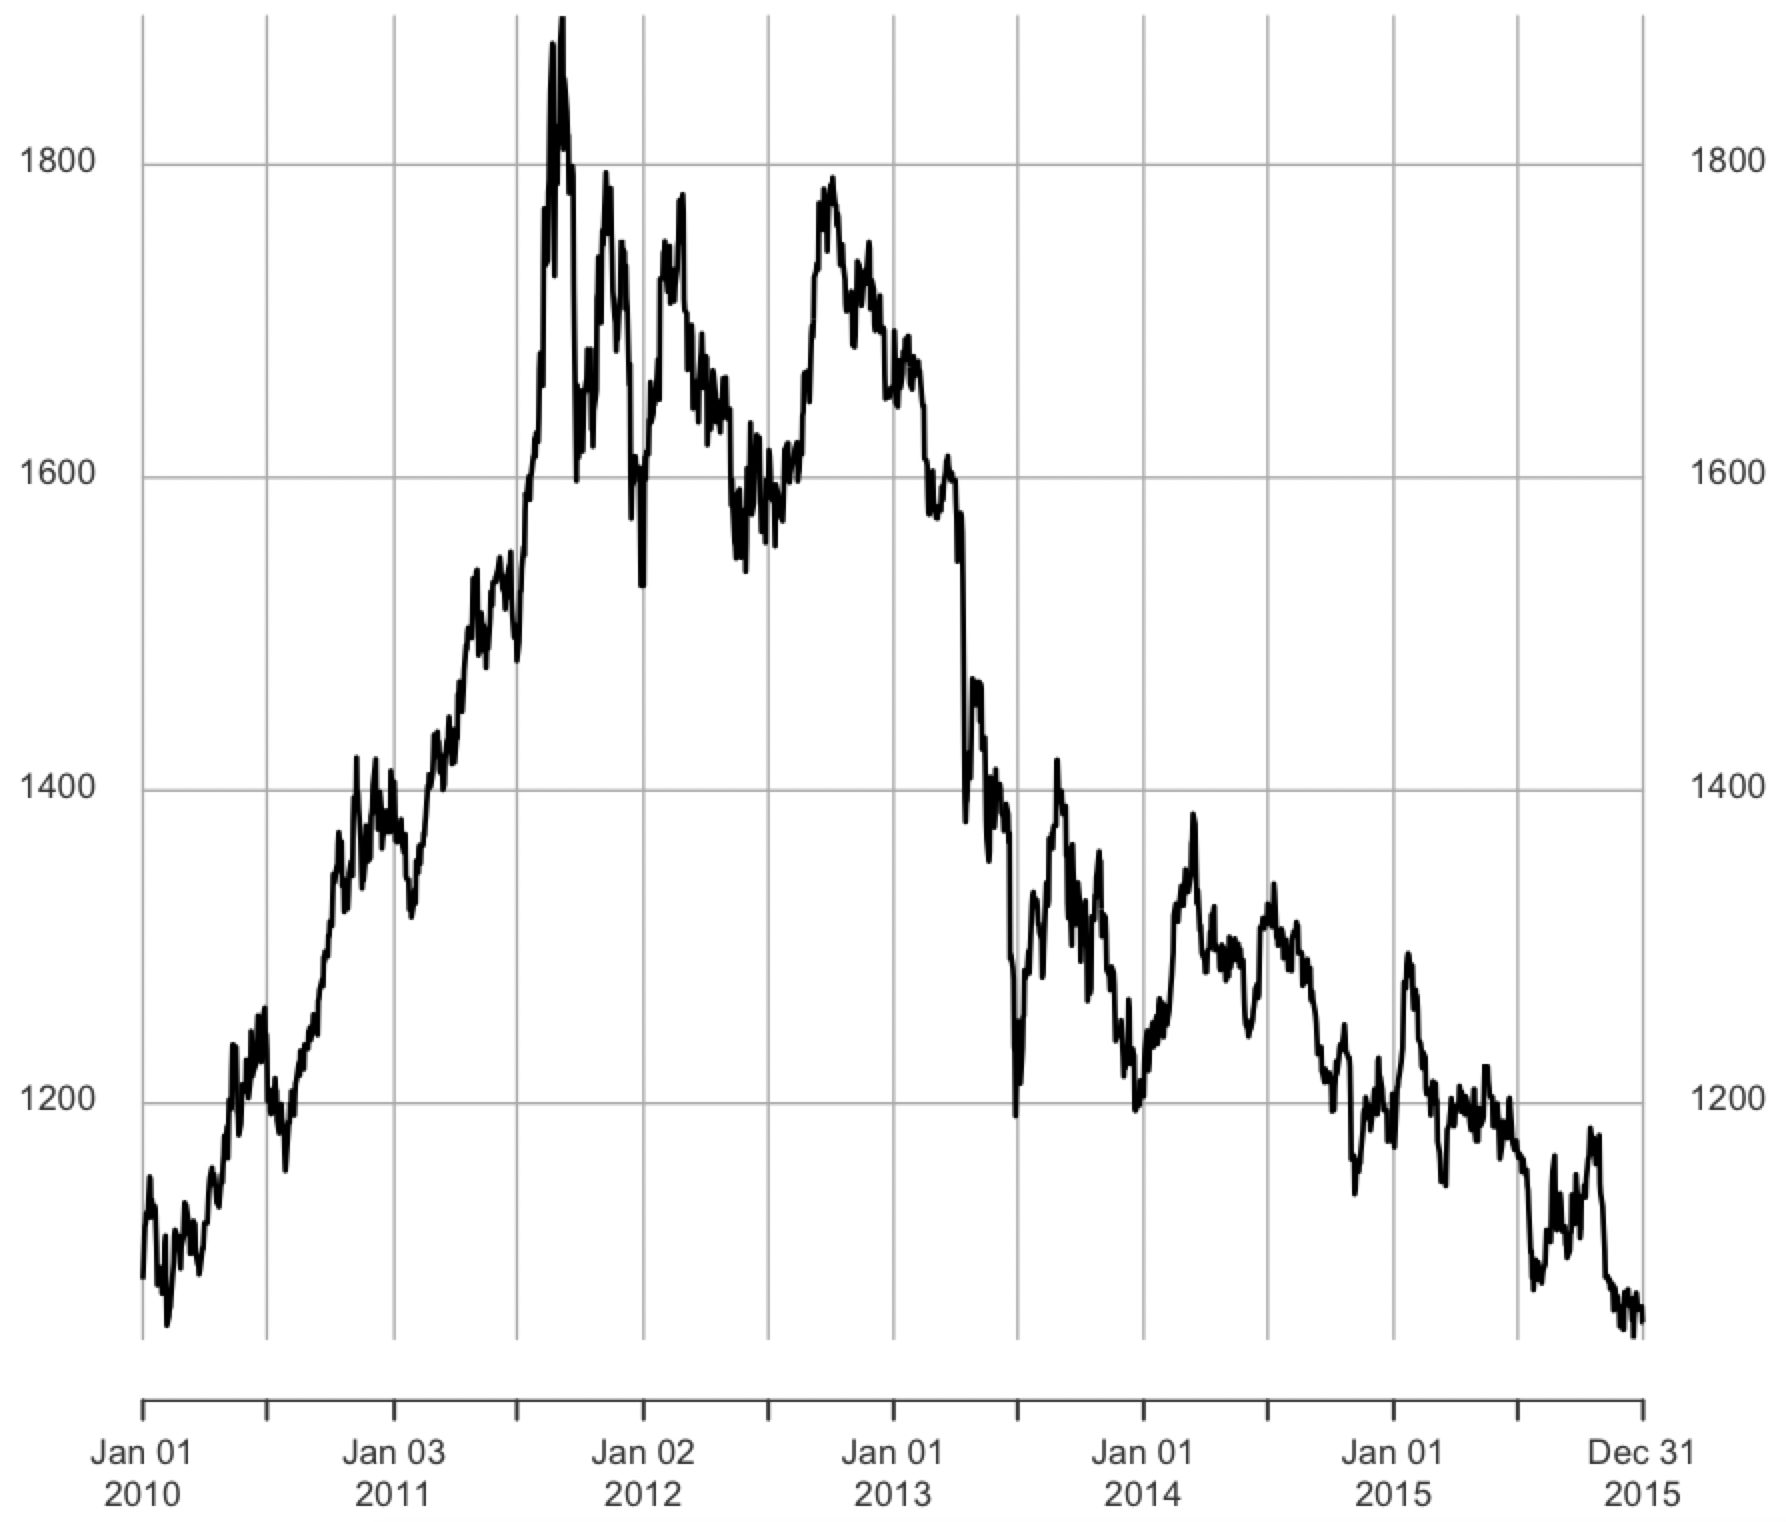
\includegraphics[width=0.6\textwidth]{data}
    \caption{Вартість золота в період з 2010 по 2015 років}
    \label{fig:data}
\end{figure}

\subsection{Аналіз даних}
Для перевірки ряду на стаціонарність було побудовано гістограму вихідного ряду (рисунок~\ref{fig:hist}).

\begin{figure}[H]
    \centering
        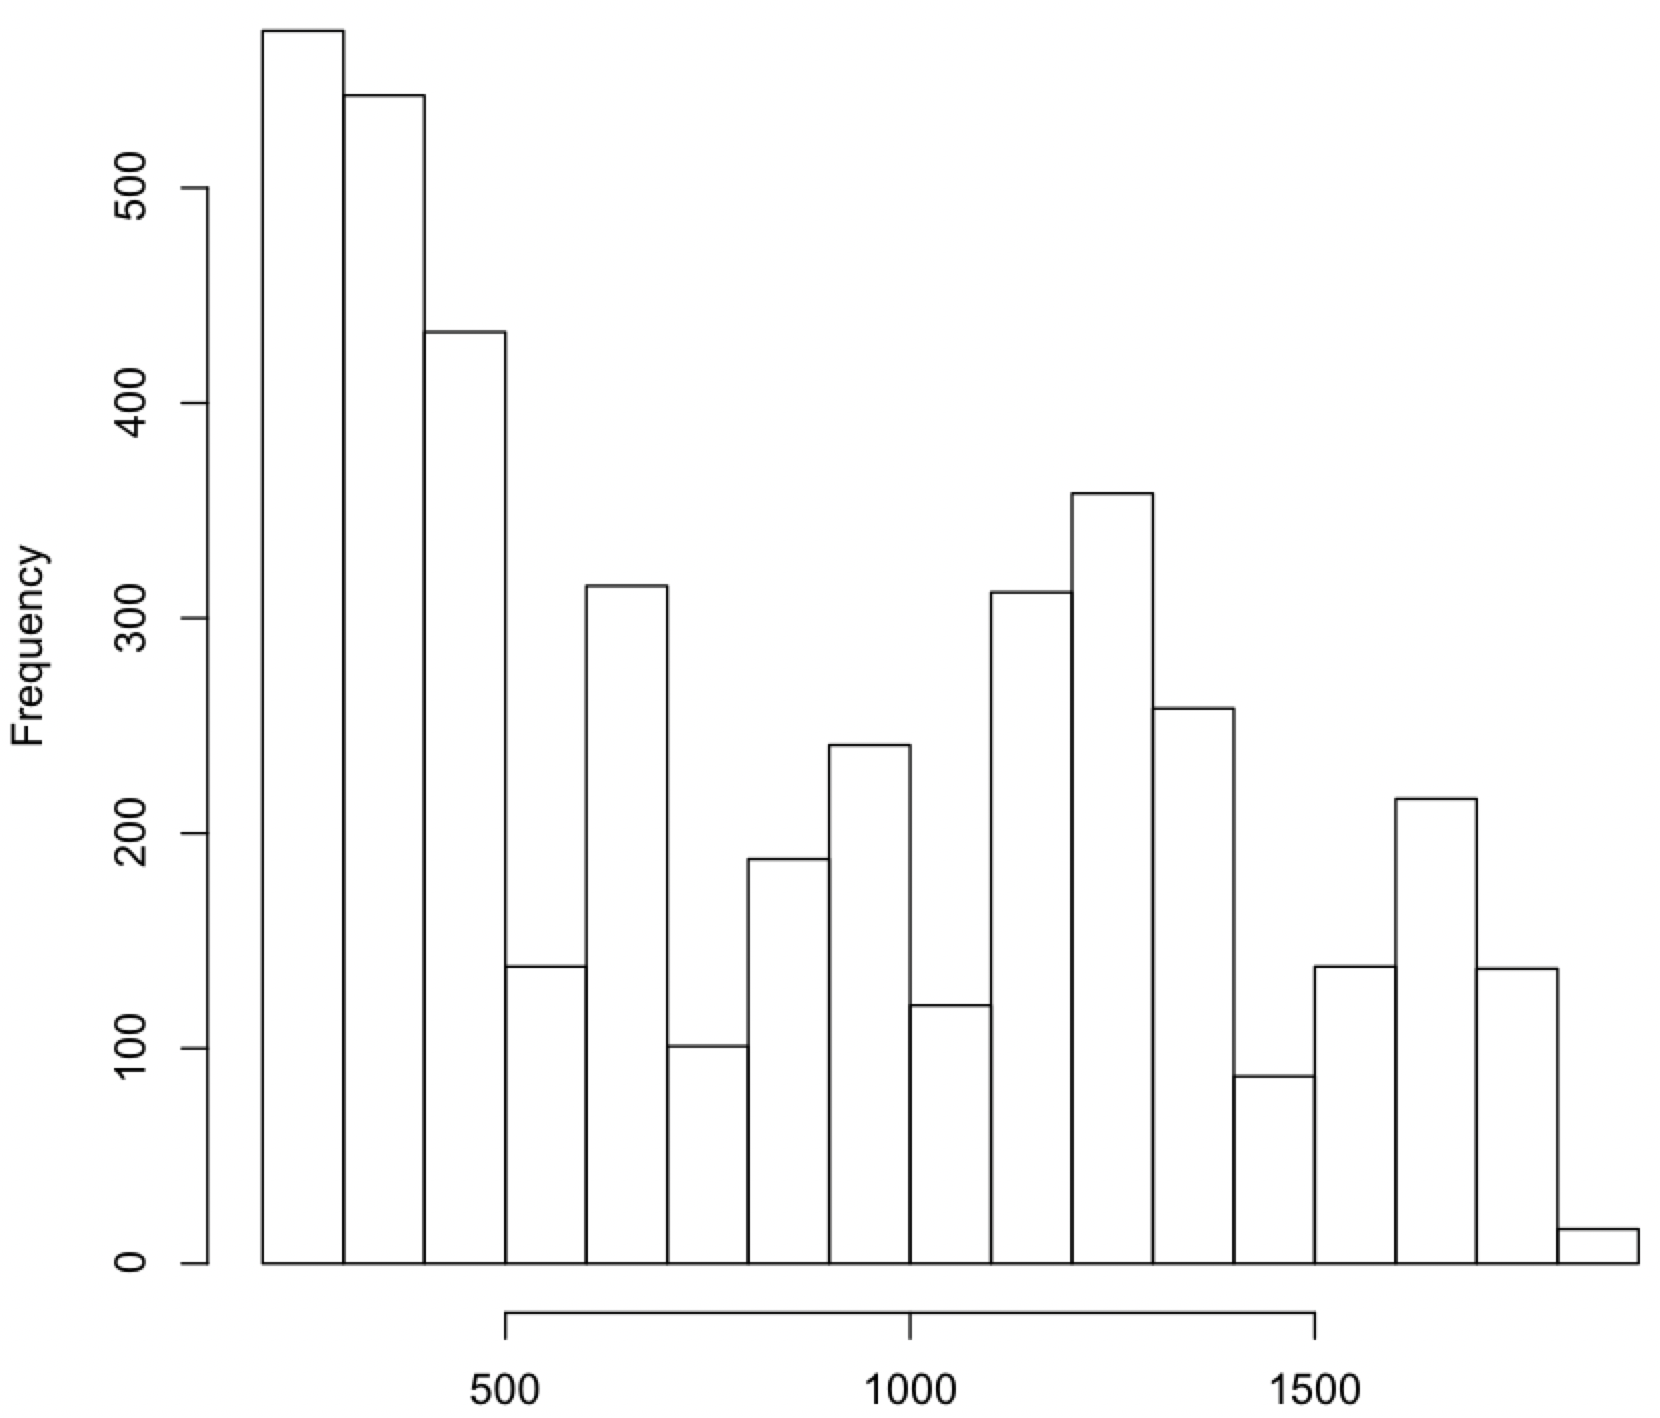
\includegraphics[width=0.6\textwidth]{hist}
    \caption{Гістограма вихідного ряду}
    \label{fig:hist}
\end{figure}

Закон разподілення вихідного ряду відрізняється від нормального а отже необхідно використовувати непараметричні тести для перевірки стаціонарністі ряду.

\subsubsection{Тест Дікі-Фулера}
Результат виконання теста:  
\begin{lstlisting}
> adf.test(data, alternative = "stationary") 

Augmented Dickey-Fuller Test
Dickey-Fuller = -0.77188, 
Lag order = 16, 
p-value = 0.9642
\end{lstlisting}

Оскільки значення $\textup{p-value} > 0.05$, то можно вважати цей ряд нестаціонарним. 

\subsection{Розробка моделі прогнозування}
Для приведення данного часового ряду до стаціонарного виду, була застосована логарифмічна трансформація та здвиг на першу різницю (рисунок~\ref{fig:temp}).  

\begin{figure}[H]
    \centering
        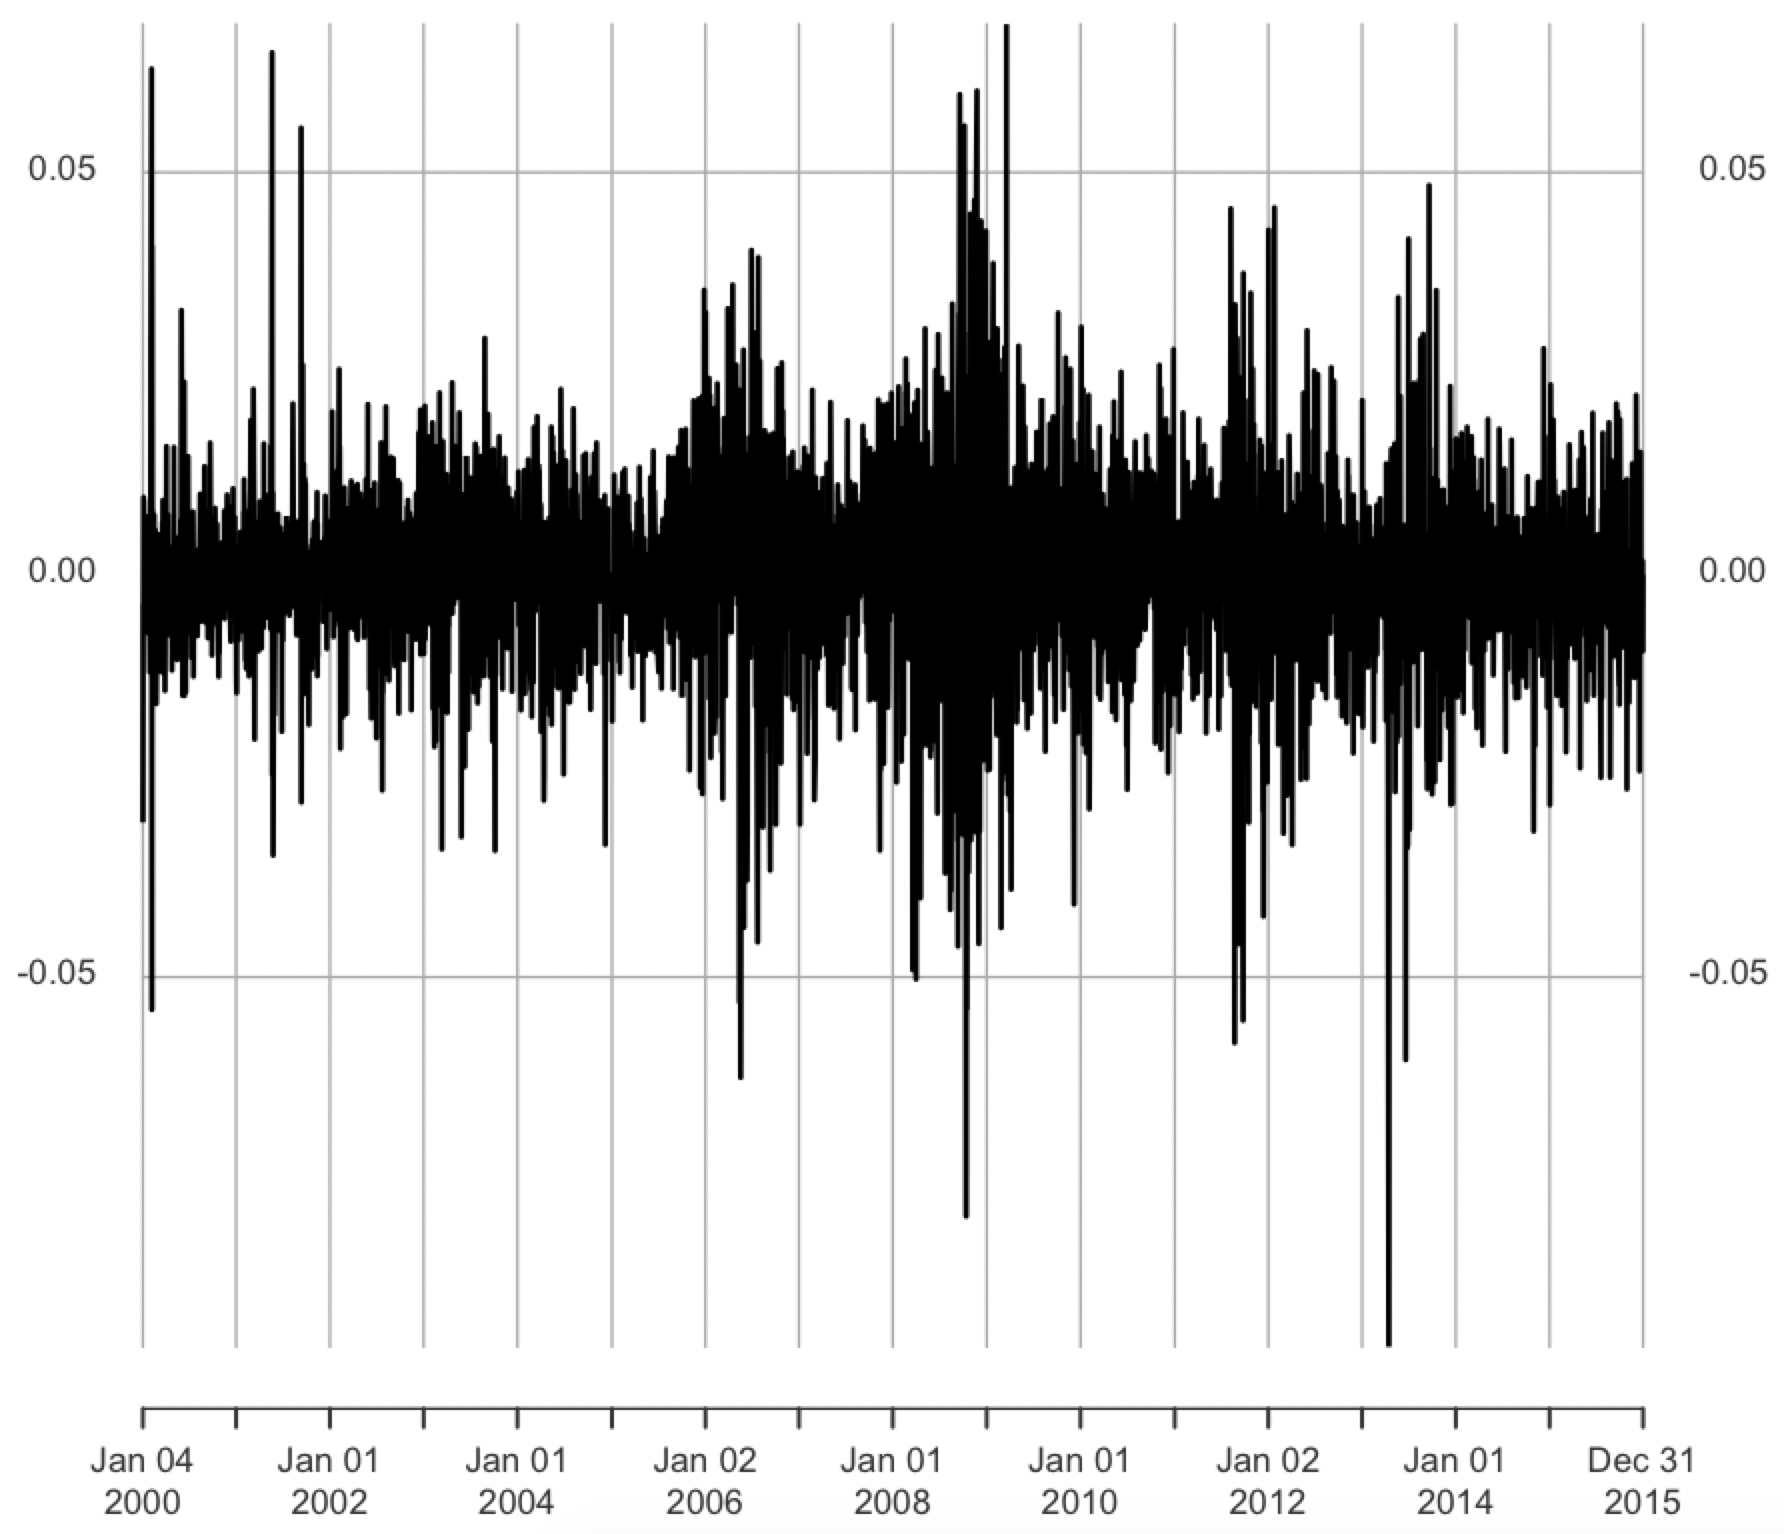
\includegraphics[width=0.6\textwidth]{temp}
    \caption{Вихідний ряд у стаціонарному виді}
    \label{fig:temp}
\end{figure} 

Проведено тест Дікі-Фулера, який показав, що даний ряд є стаціонарним:
\begin{lstlisting}
> adf.test(data, alternative = "stationary") 

Augmented Dickey-Fuller Test
Dickey-Fuller = -16.169, 
Lag order = 16, 
p-value = 0.01
\end{lstlisting}

\subsection{Прогнозування}
\subsubsection{ARIMA}
Результат прогнозування за допомогою метода ARIMA з використанням бібліотеки \texttt{forecast} зображено на рисунку~\ref{fig:out_arima}.  

\begin{figure}[H]
    \centering
        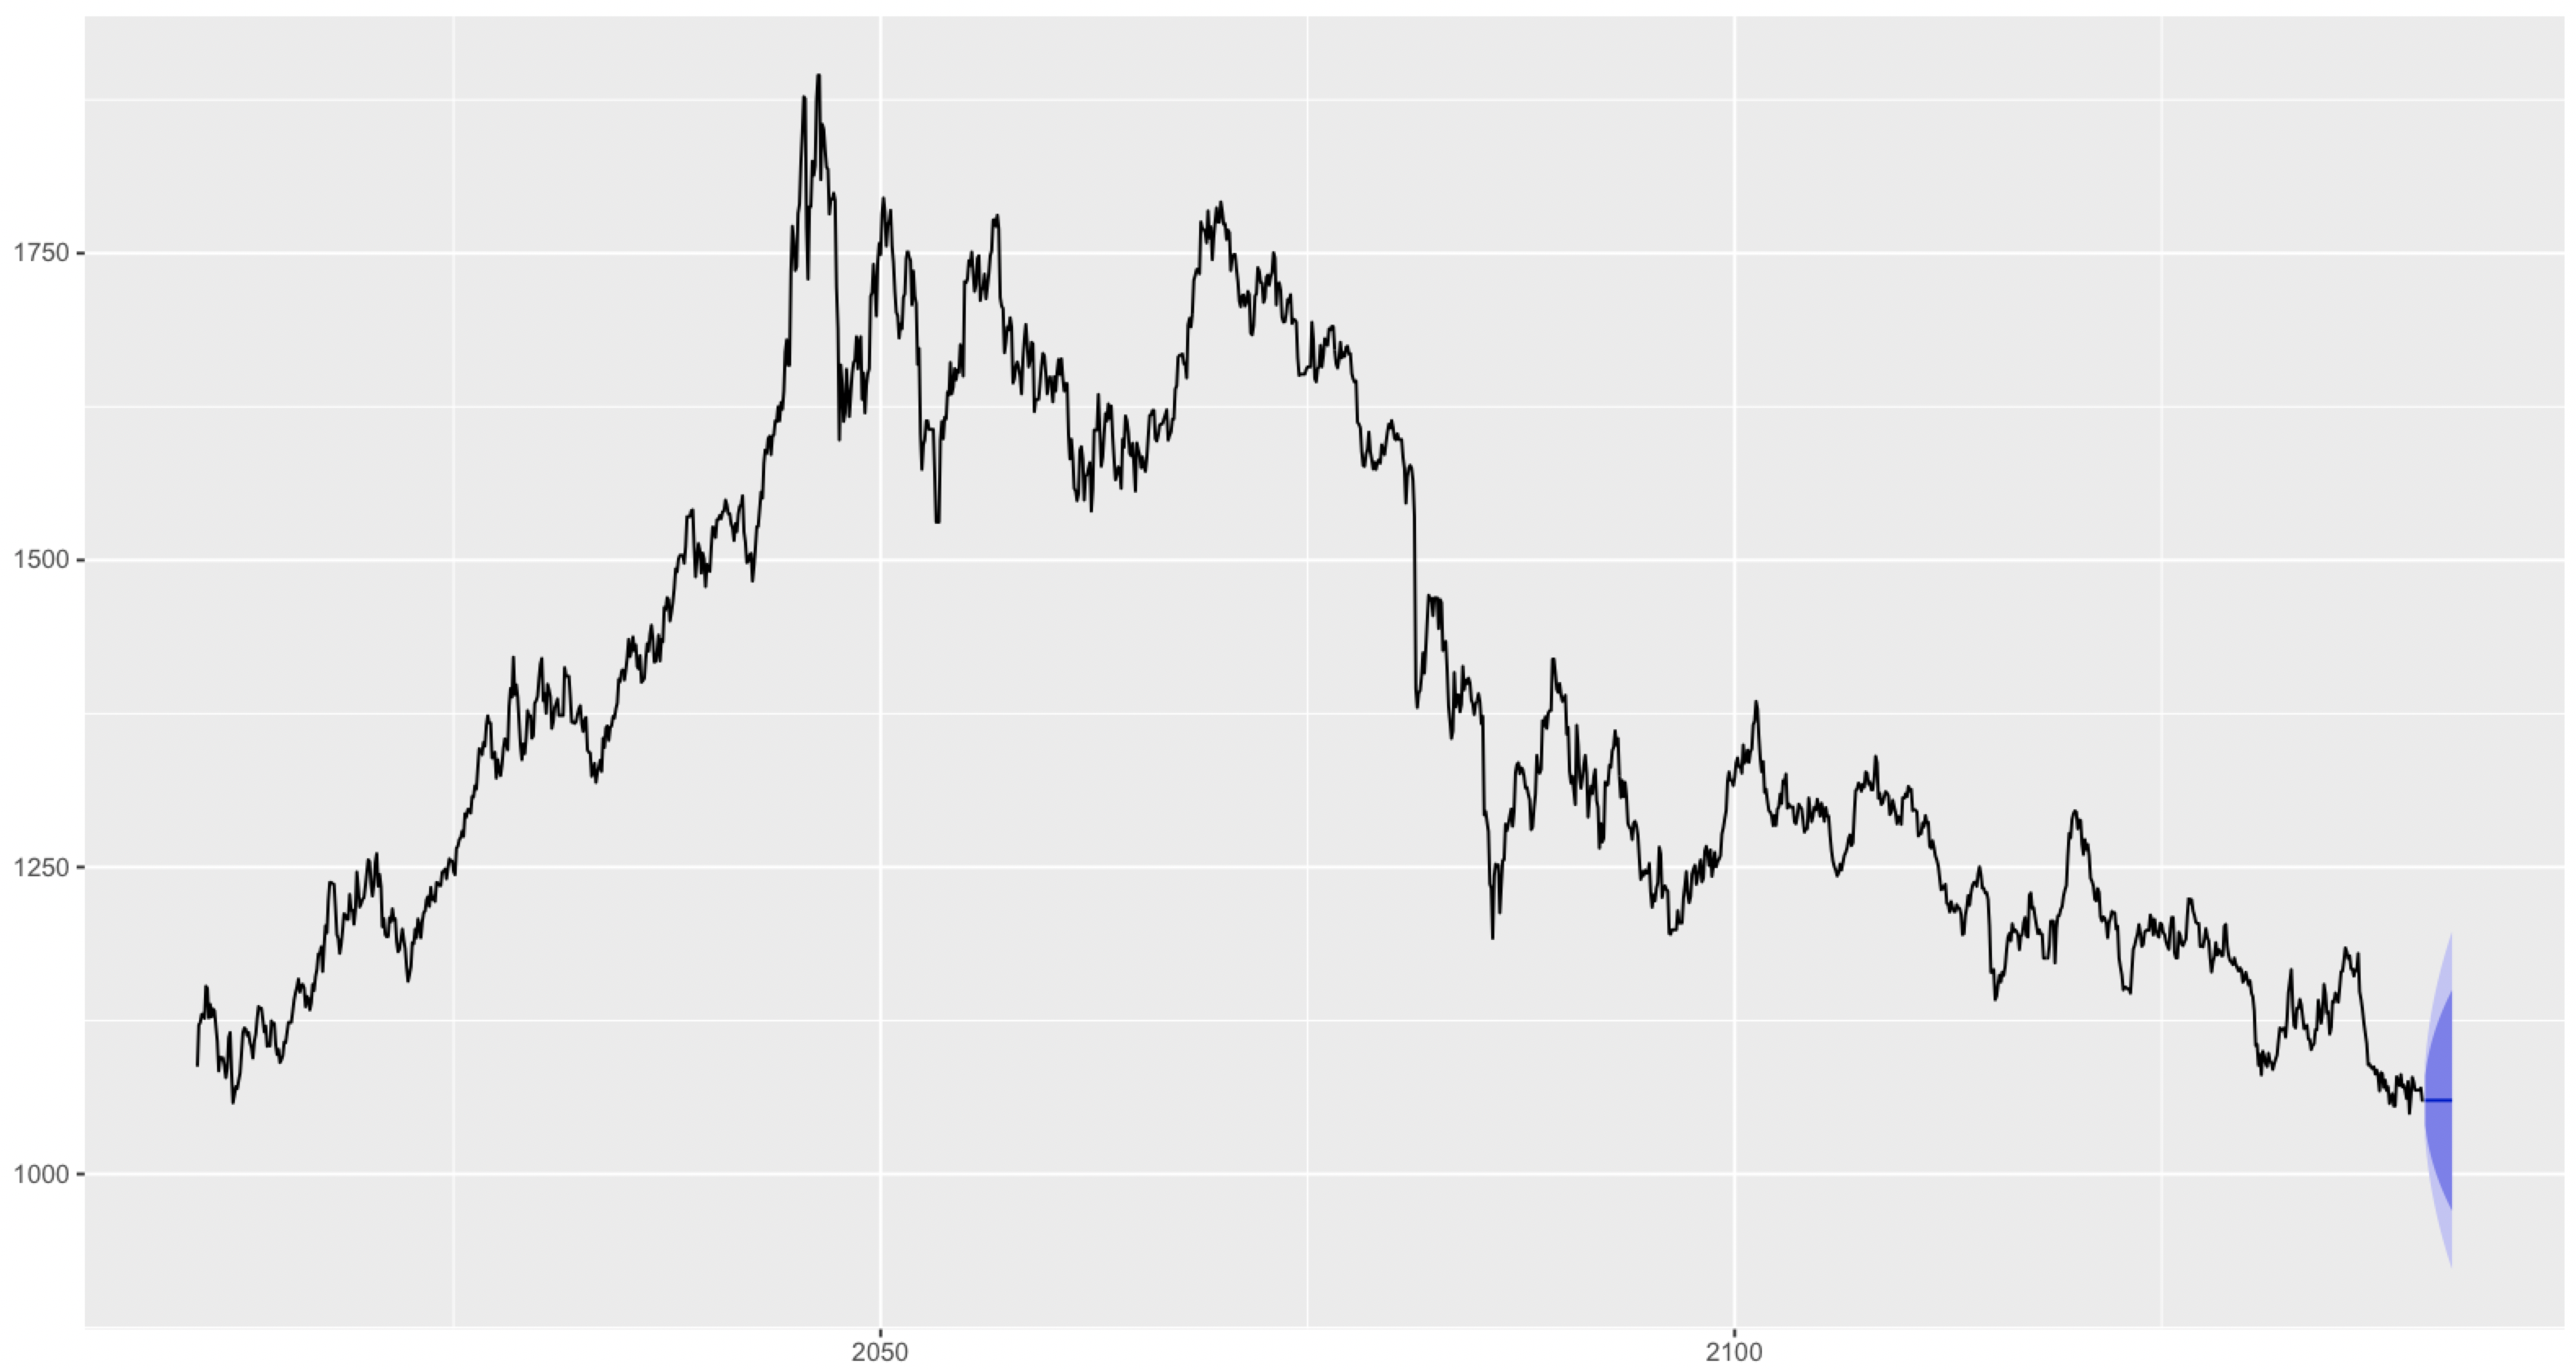
\includegraphics[width=1\textwidth]{out_arima}
    \caption{ARIMA}
    \label{fig:out_arima}
\end{figure} 

\subsubsection{ARFIMA}
Результат прогнозування за допомогою метода ARFIMA з використанням бібліотеки \texttt{forecast} зображено на рисунку~\ref{fig:out_arfima}.  

\begin{figure}[H]
    \centering
        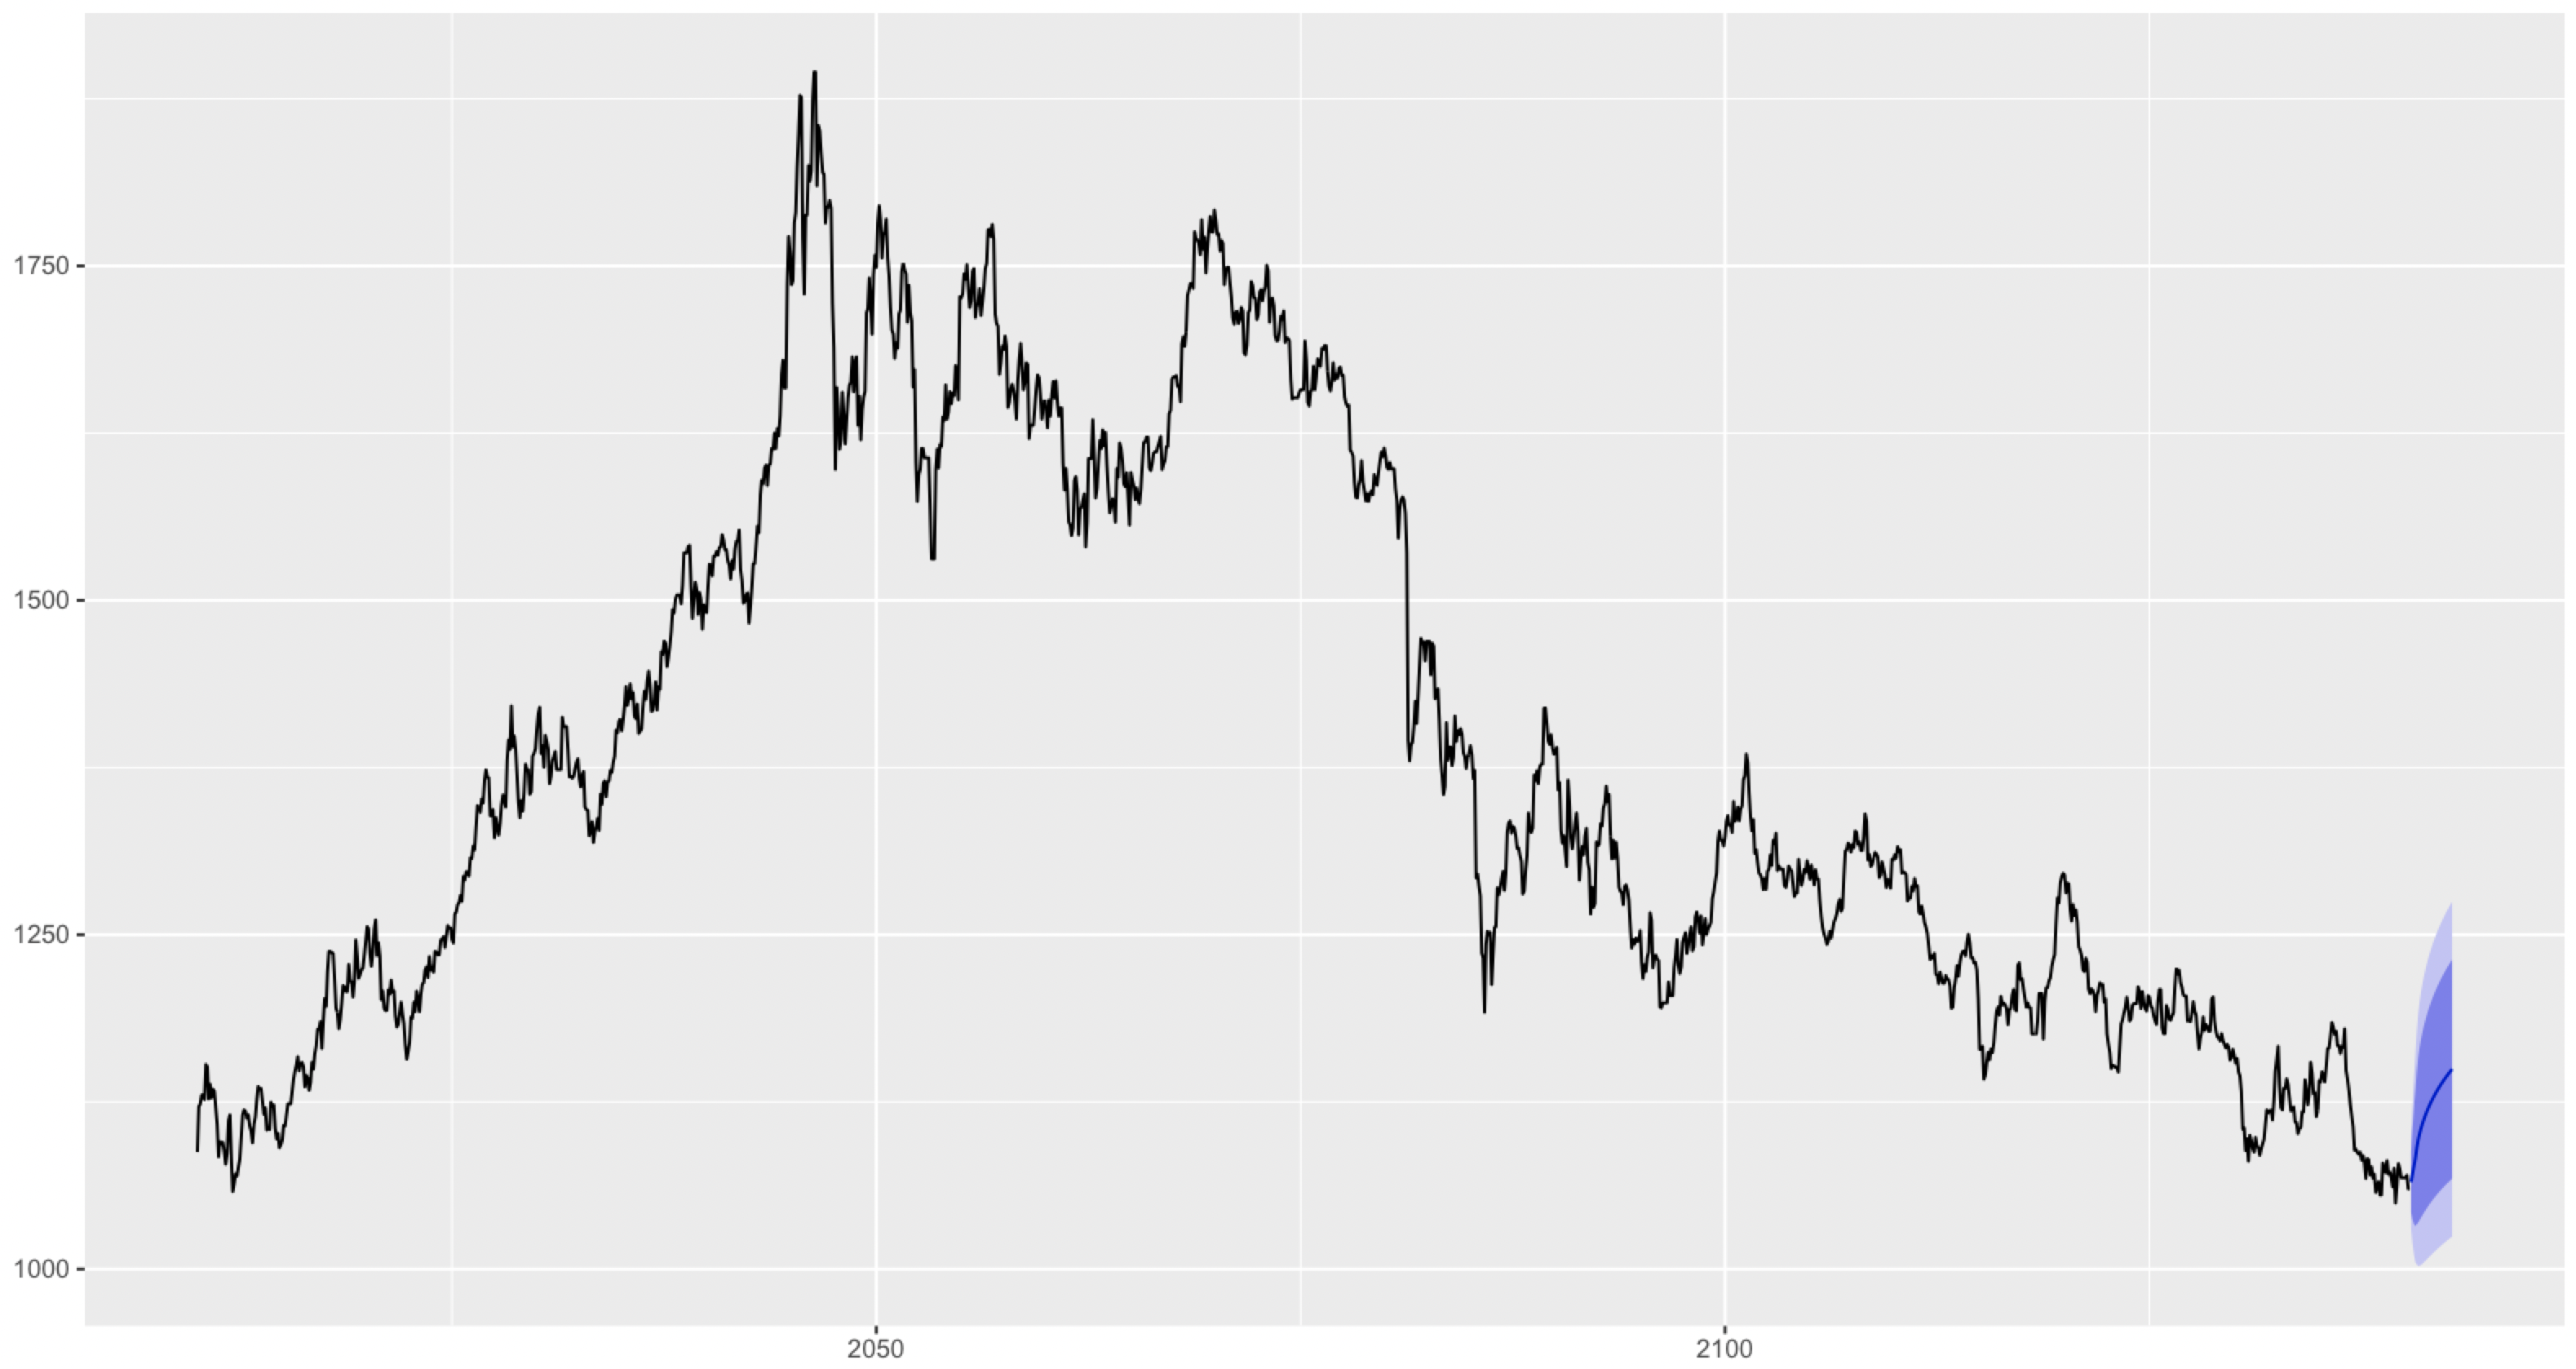
\includegraphics[width=1\textwidth]{out_arfima}
    \caption{ARFIMA}
    \label{fig:out_arfima}
\end{figure} 

\subsubsection{TBATS}
Результат прогнозування за допомогою метода TBATS з використанням бібліотеки \texttt{forecast} зображено на рисунку~\ref{fig:out_tbats}.  

\begin{figure}[H]
    \centering
        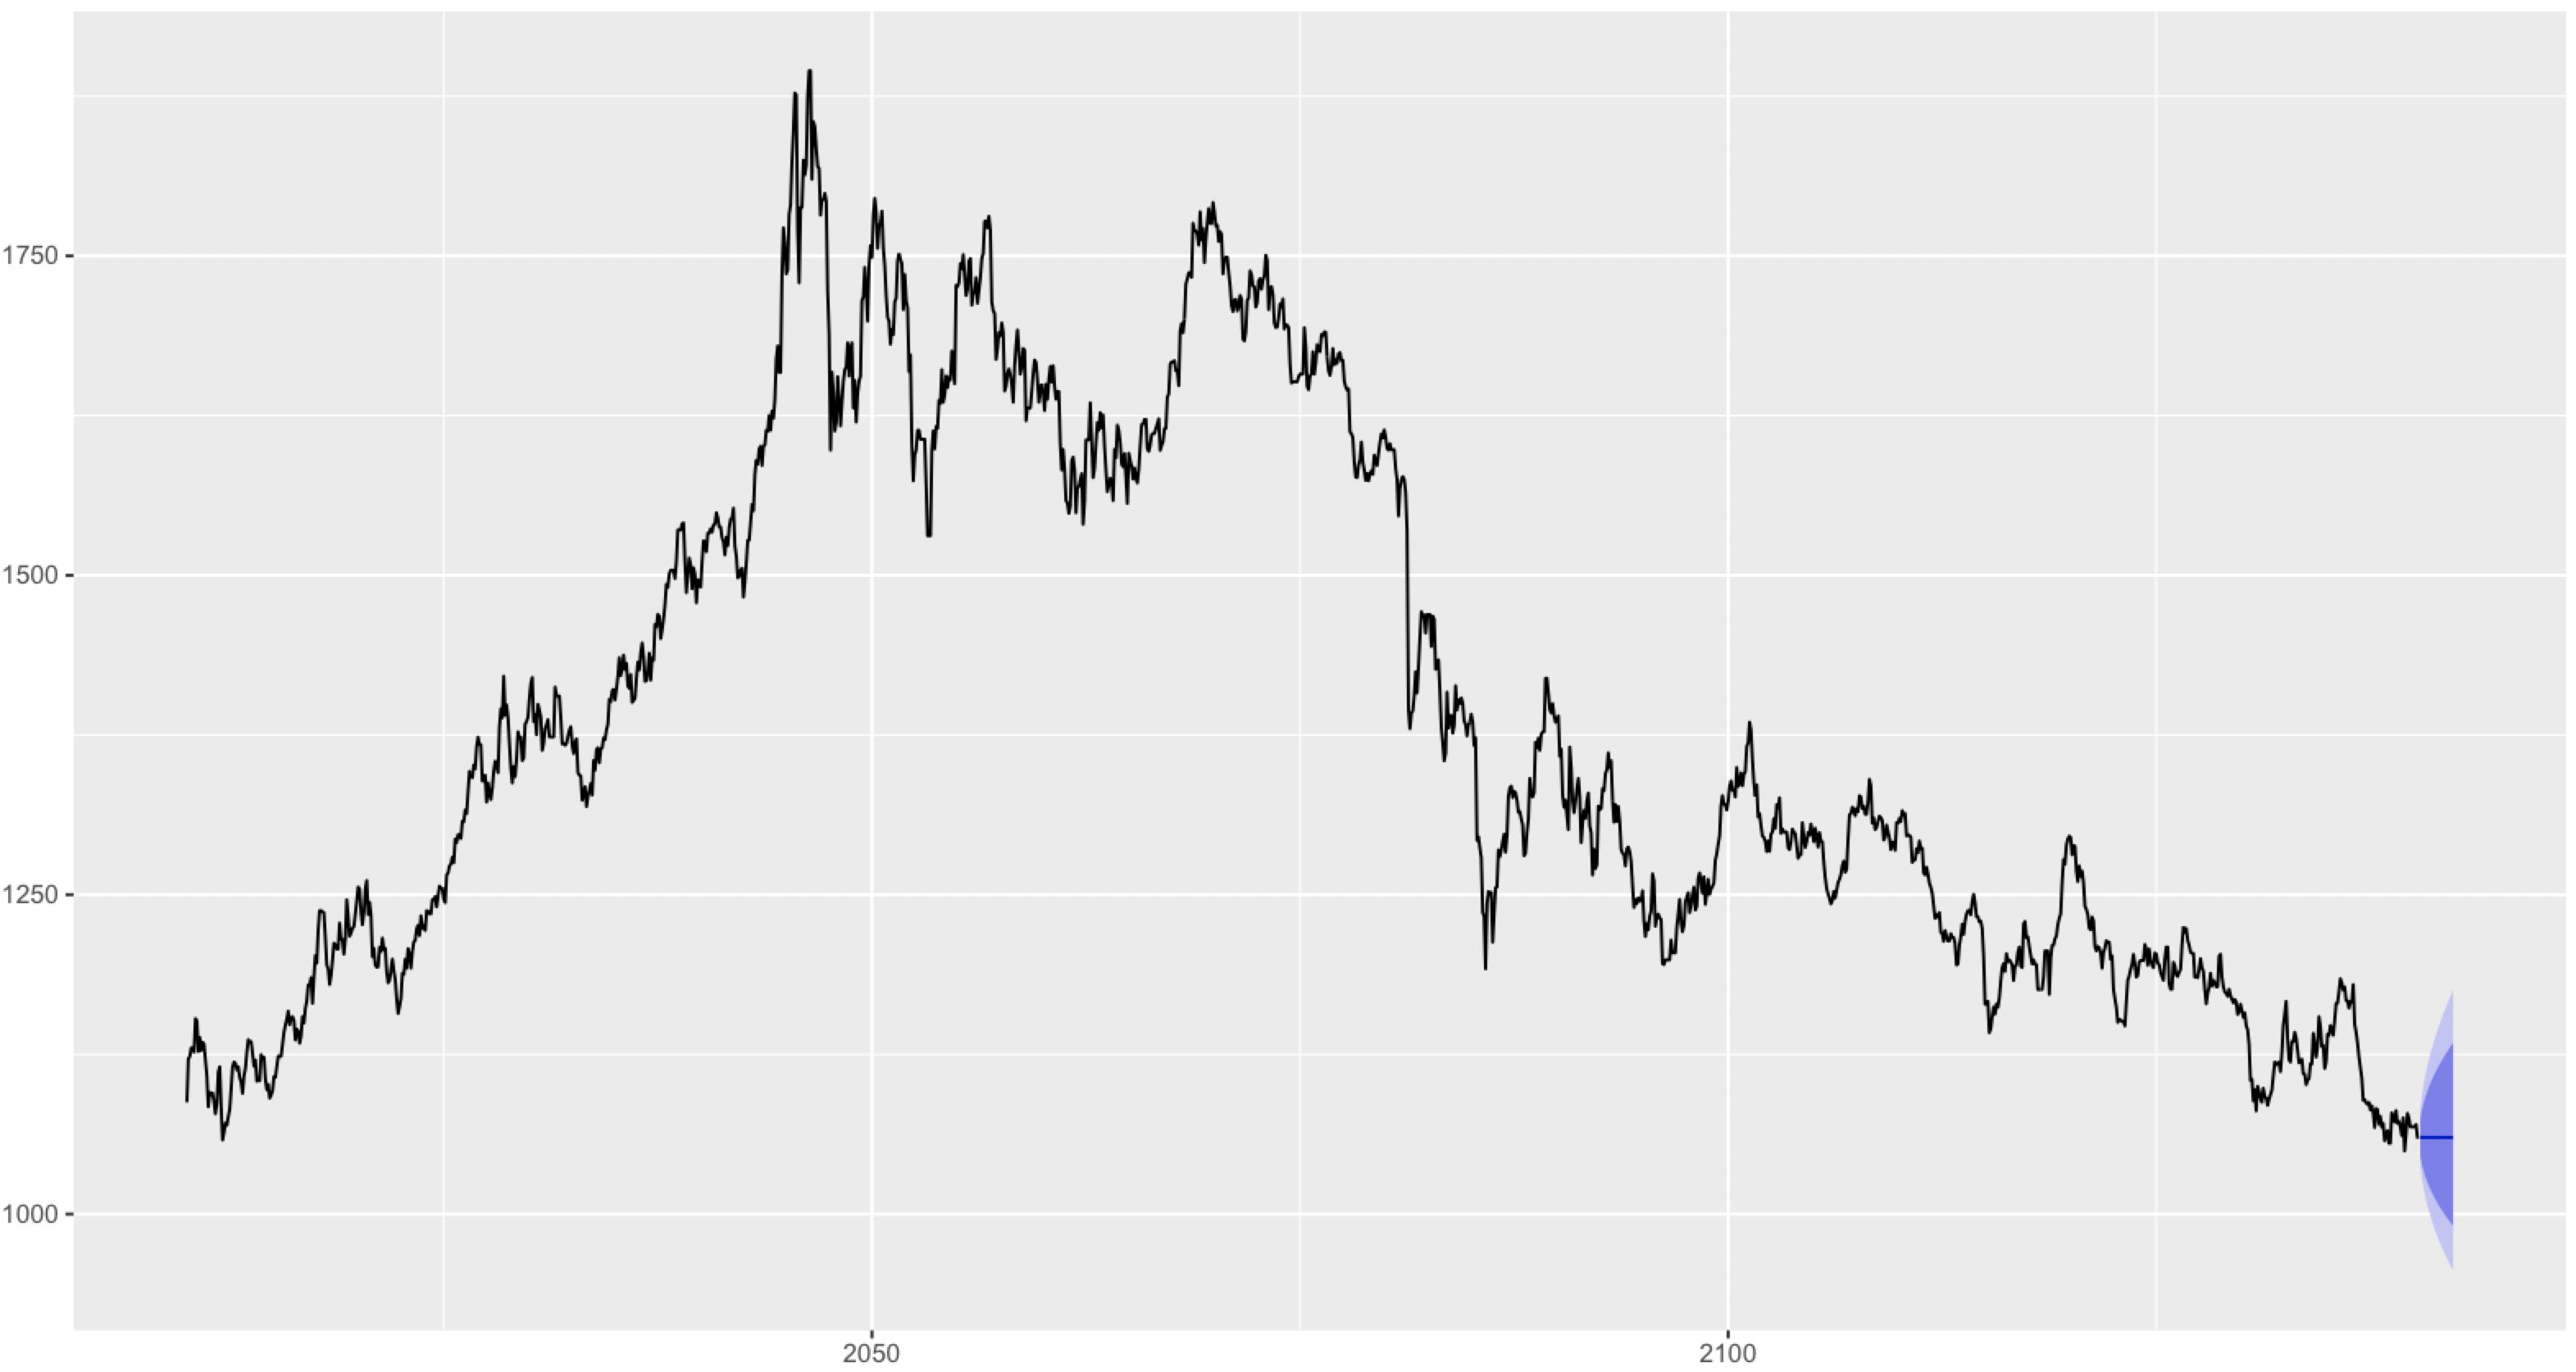
\includegraphics[width=1\textwidth]{out_tbats}
    \caption{TBATS}
    \label{fig:out_tbats}
\end{figure} 

\subsection{Розробка веб-додатку}
Макет додатку представлено на рисунку~\ref{fig:app_mockup}.\\[0.3em]

\begin{figure}[H]
    \centering
        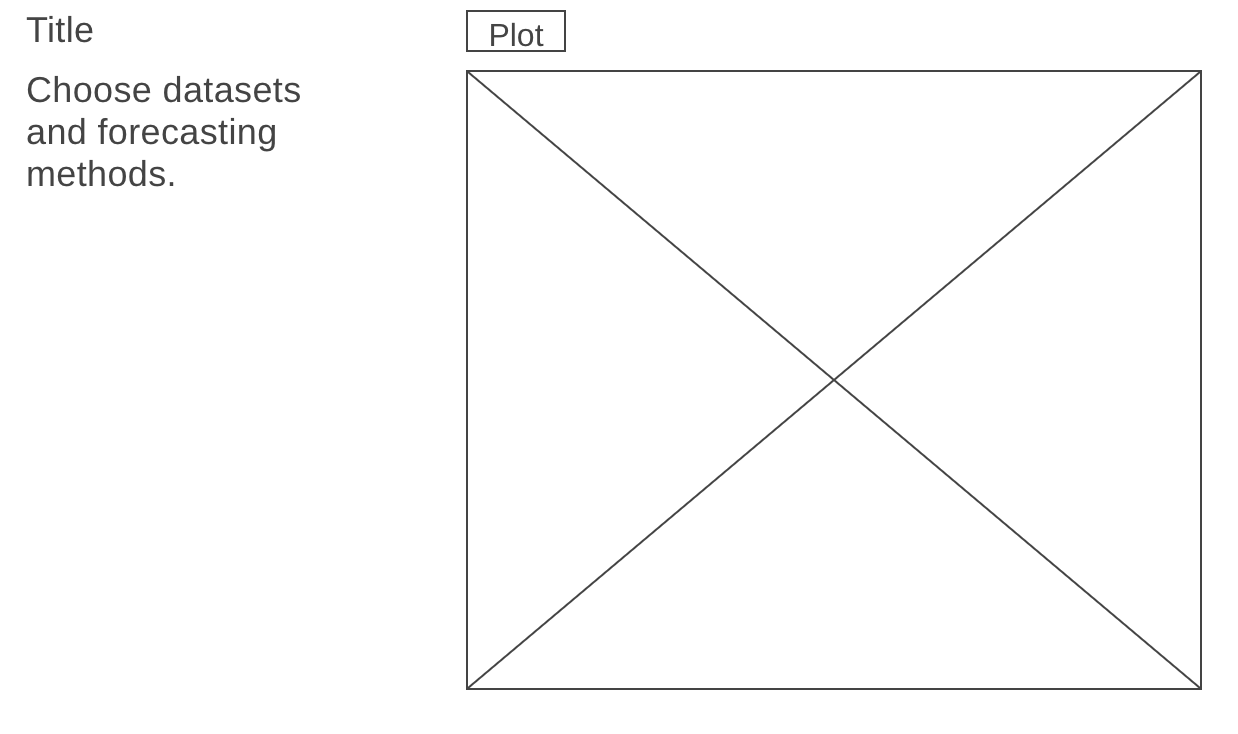
\includegraphics[width=0.6\textwidth]{app_mockup}
    \caption{Макет додатку}
    \label{fig:app_mockup}
\end{figure} 

У якості даних було обрано вартість золота, GBP, EUR, CAD та популярні криптовалюти BTC, ETH, XRP. 
У якості методів прогнозування було обрано ETS, ARIMA, ARFIMA, TBATS.

Код веб-додатку:
\lstinputlisting{code/main.r}

Скріншот веб-додатку представлений на рисунку~\ref{fig:app_screen}.

\begin{figure}[H]
    \centering
        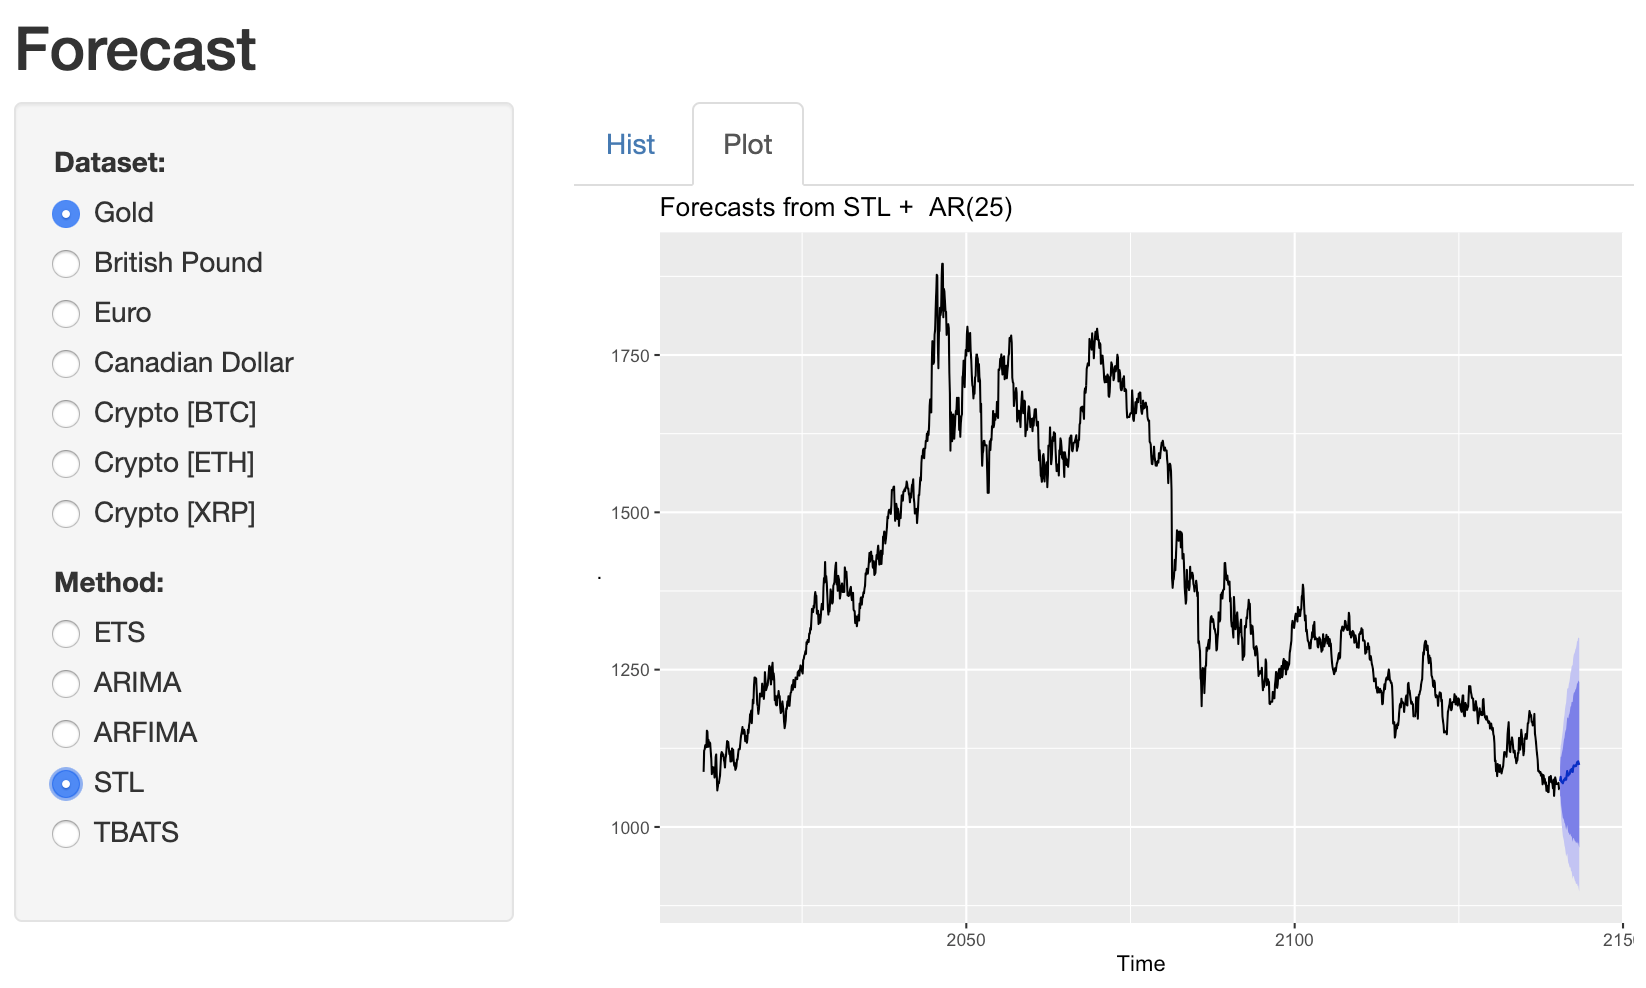
\includegraphics[width=1\textwidth]{app_screen}
    \caption{Скріншот додатку}
    \label{fig:app_screen}
\end{figure} 

\subsection*{Висновки}
У ході виконання розрахунково-графічного завдання було виконано аналіз числового ряду вартості золота, побудовано прогноз числового ряду за допомогою методів ETS, ARIMA, ARFIMA, TBATS. 

Мова програмування R добре підходить для таких задач, та має багато готових к використанню бібліотек. 

\end{document}
